\documentclass[
  english,            % define the document language (english, german)
  aspectratio=169,    % define the aspect ratio (169, 43)
  % handout=2on1,       % create handout with multiple slides (2on1, 4on1)
  % partpage=false,     % insert page at beginning of parts (true, false)
  % sectionpage=true,   % insert page at beginning of sections (true, false)
]{tumbeamer}

\usepackage[export]{adjustbox}
\usepackage{amsmath}
\usepackage{wrapfig}
\usepackage{graphicx}
\usepackage{blindtext}
\usepackage{listings}
\usepackage{amssymb}
\usepackage{float}
\usepackage{tikz}
\usepackage{pgfplots}
\usepackage{caption}
\pgfplotsset{compat=newest}
\usepackage{color}
\usepackage{booktabs}
\usepackage{pifont}


\title{Practical Course Data Structure Engineering}
\subtitle{Group 11 \\ The Tandem Counting Bloomfilter}
\author{Cong Thanh Dang | Thua Duc Nguyen}
\date[07/02/2024]{Wintersemester 2023/2024}
\footline{\insertauthor~|~\insertshorttitle~|~\insertshortdate}

\TUMbeamersetup{
  title page = TUM tower,         % style of the title page
  part page = TUM toc,            % style of part pages
  section page = TUM toc,         % style of section pages
  content page = TUM more space,  % style of normal content pages
  tower scale = 1.0,              % scaling factor of TUM tower (if used)
  headline = TUM threeliner,      % which variation of headline to use
  footline = TUM default,         % which variation of footline to use
  % configure on which pages headlines and footlines should be printed
  headline on = {title page},
  footline on = {every page, title page=false},
}

\begin{document}

\maketitle

\section{Benchmarking}

\begin{frame}{Benchmarking}{Test environment}
    \begin{itemize}
        \item \textbf{Processor:} 10th Gen Intel\textsuperscript{\textregistered} Core\texttrademark~i7-1065G7 @ 3.900GHz $\times$ 4
        \item \textbf{Operating System:} Arch Linux x86\_64
        \item \textbf{Compiler:} clang++ std=20 with O3
    \end{itemize}
\end{frame}    

\begin{frame}{Benchmarking}{Set up}
        \textbf{Test parameter:} 
            \begin{itemize}
                    \item Filter length: $m = 16384$ bits (2048 bytes)
                    \item Num of hash functions $k = 4$
                    \item Variable increment parameter $L = 8$
                    \item Number of repetitions $r = 5$
            \end{itemize}
\end{frame}


\begin{frame}{Benchmarking}{Runtime}
        \begin{itemize}
            \item Insert $100.000$ items to filter
            \item Lookup $100.000$ items
            \item Remove $100.000$ items from filter
        \end{itemize}
\end{frame}

\begin{frame}{Benchmarking}{Runtime}
    \vspace{-10pt}
    \begin{figure}
    \centering
    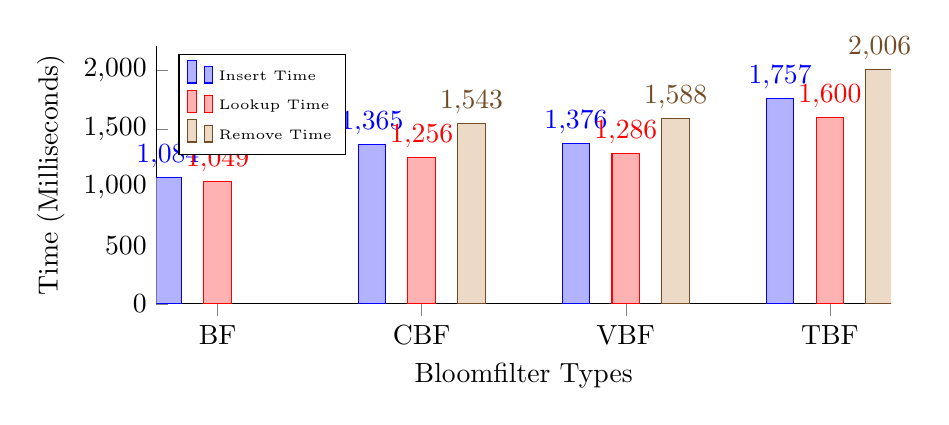
\begin{tikzpicture}
        \begin{axis}[
            ybar,
            width = 0.9\textwidth,
            height = 0.4\textwidth,
            xlabel={Bloomfilter Types},
            ylabel={Time (Milliseconds)},
            symbolic x coords={BF, CBF, VBF, TBF},
            xtick=data,
            ymin = 0,
            nodes near coords,
            nodes near coords align={vertical},
            legend pos=north west,
            legend style={
                font=\tiny, cells={anchor=west},
                /tikz/every even column/.append style={column sep=0.5cm}
            },
            ybar=8pt,
            bar width=10pt,
            axis lines*=left
        ]
        
        % Insert times
        \addplot coordinates {(BF, 1084) (CBF, 1365) (VBF, 1376) (TBF, 1757)};
        % Lookup times
        \addplot coordinates {(BF, 1049) (CBF, 1256) (VBF, 1286) (TBF, 1600)};
        % Remove times
        \addplot coordinates {(BF, NaN) (CBF, 1543) (VBF, 1588) (TBF, 2006)};
        
        \legend{Insert Time, Lookup Time, Remove Time}
        \end{axis}
    \end{tikzpicture}
    \label{fig:benchmark}
    \end{figure}
\end{frame}

\begin{frame}{Benchmarking}{False positive rate}

    \begin{table}[h]
        \begin{tabular}{|c|c|c|c|c|c|c|}
            \hline
            Inserted items & 820 & 683 & 586 & 512 & 456 & 410 \\
            \hline
            Bits per element & 40 & 48 & 56 & 64 & 72 & 80 \\
            \hline
        \end{tabular}
        \label{tab:items}
    \end{table}
    
    \textbf{Test No Removal}:
    \begin{itemize}
        \item Insert randomly the above amount items
        \item Check randomly $100.000$ other items that not inserted
    \end{itemize}
    \vspace{5pt}
    \textbf{Test Removal Block}:
    \begin{itemize}
        \item Insert randomly the above amount items
        \item Insert and delete immediately the above amount items
        \item Check randomly $100.000$ other items that not inserted
    \end{itemize}
\end{frame}


\begin{frame}{Benchmarking}{False positive possibility}
  \begin{figure}
    \centering
    \vspace{-10pt}
    \begin{tikzpicture}
      \begin{axis}[
          width = 0.9\textwidth,
          height = 0.45\textwidth,
          xlabel={Bits per element},
          ylabel={False Positive Rate (\%)},
          grid=major,
          legend pos=south west,
          legend style={
            font=\tiny, cells={anchor=west},
            /tikz/every even column/.append style={column sep=0.5cm}
          },
          ymin=0.0001, % set the minimum value of y-axis
          ymax=1, % set the maximum value of y-axis
          ymode=log, % this will set the y-axis to logarithmic scale
          log basis y={10}, % the base of the logarithm (default is 10)
          ytick={1,0.1,0.01,0.001,0.0001},
          yticklabels={$1$,$10^{-1}$,$10^{-2}$,$10^{-3}$,$10^{-4}$},
          major grid style={lightgray},
          minor grid style={lightgray!25},
          minor y tick num=1, 
          xtick={40, 
          48, 56, 64, 72, 80},
          xticklabel={\pgfmathprintnumber{\tick}}
        ]
        \addplot[mark=square*, smooth, thick, blue] file{data/cbf_fpr.dat};
        \addlegendentry{Counting Bloomfilter}
        
        \addplot[mark=triangle*, smooth, thick, orange] file{data/vbf_fpr.dat};
        \addlegendentry{Variable Couting Bloomfilter}
        
        \addplot[mark=diamond*, smooth, thick, red] file{data/tbf_fpr.dat};
        \addlegendentry{Tandem Couting Bloomfilter}
        
        \addplot[mark=triangle*, smooth, thick, black, dotted] file{data/vbf_blockremoval.dat};
        \addlegendentry{Variable Couting Bloomfilter - Block removal}
        
        \addplot[mark=diamond*, smooth, thick, green, dotted] file{data/tbf_blockremoval.dat};
        \addlegendentry{Tandem Couting Bloomfilter - Block removal}
      
      \end{axis}
    \end{tikzpicture}
  \end{figure}
\end{frame}


\begin{frame}{Benchmarking}{False positive improvement}
  \begin{figure}
    \centering
    \vspace{-10pt}
    \begin{tikzpicture}
      \begin{axis}[
          width = 0.9\textwidth,
          height = 0.45\textwidth,
          xlabel={Bits per element},
          ylabel={False positive rate improvement},
          legend pos=north west,
          legend style={
            font=\tiny, cells={anchor=east},
            /tikz/every even column/.append style={column sep=0.5cm}
          },
          ymin=0,
          ymax=18,
          grid = both,
          ytick={2,4,6,8,10,12,14,16,18},
          yticklabel={\pgfmathprintnumber{\tick}},
          xtick={40, 48, 56, 64, 72, 80},
          xticklabel={\pgfmathprintnumber{\tick}}
      ]
      \addplot[mark=diamond*, smooth, thick, red] file{data/factor.dat};
      \addlegendentry{TBF to VI-CBF}
      \addplot[mark=square*, smooth, thick, blue] file{data/factor_removal.dat};
      \addlegendentry{TBF Removal to VI-CBF Removal}
      \end{axis}
    \end{tikzpicture}
  \end{figure}
\end{frame}

\section{Surprising findings}
\begin{frame}{Surprising findings}{Insertion mistake}
  \begin{minipage}{0.5\textwidth}
    \includegraphics[width=\linewidth]{img/tbf_insertion_text_mark.pdf}
    \captionof{figure}{Description of insertion}
  \end{minipage}
  \begin{minipage}{0.35\textwidth}
    \includegraphics[width=\linewidth]{img/tbf_insertion_pseudo_mark.pdf}
    \captionof{figure}{Pseudocode of insertion}
  \end{minipage}
\end{frame}

\begin{frame}{Surprising findings}{Why?}
    \begin{itemize}
        \item $L=4, k=1$
        \item $v_{g_{1}{(y)}} = 5, w_{h_{1}{(y)}} = 1$ and $v_{g_{1}{(x)}} = 7, w_{h_{1}{(x)}} = 3$
    \end{itemize}

\bigskip

\begin{minipage}{0.4\textwidth}
\textit{Expected:}
\centering
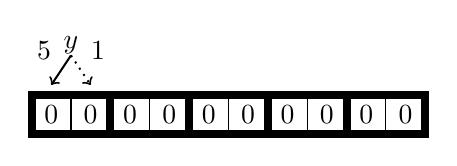
\begin{tikzpicture}[scale=0.5]
  \foreach \x in {0,1,...,9}
    \draw (\x,0) rectangle (\x+1,1);
   \foreach \x/\num in {0.5/0,1.5/0,2.5/0,3.5/0,4.5/0,5.5/0,6.5/0,7.5/0,8.5/0,9.5/0}
     \node at (\x,0.5) {\num};
  \foreach \x in {0,2,...,8}
    \draw[line width=1mm] (\x,0) rectangle (\x+2,1);
  \node at (1.0,2.25) {$y$};
  
  \draw[->, line width=0.25mm] (1.0,2.0) -- node[above left] {$5$} (0.5,1.25);
   \draw[->, dotted, line width=0.25mm] (1.0,2.0) -- node[above right] {$1$} (1.5,1.25);
\end{tikzpicture}
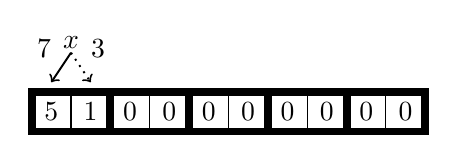
\begin{tikzpicture}[scale=0.5]
  \foreach \x in {0,1,...,9}
    \draw (\x,0) rectangle (\x+1,1);
   \foreach \x/\num in {0.5/5,1.5/1,2.5/0,3.5/0,4.5/0,5.5/0,6.5/0,7.5/0,8.5/0,9.5/0}
     \node at (\x,0.5) {\num};
  \foreach \x in {0,2,...,8}
    \draw[line width=1mm] (\x,0) rectangle (\x+2,1);

  \node at (1.0,2.25) {$x$};
  
  \draw[->, line width=0.25mm] (1.0,2.0) -- node[above left] {$7$} (0.5,1.25);
   \draw[->, dotted, line width=0.25mm] (1.0,2.0) -- node[above right] {$3$} (1.5,1.25);
\end{tikzpicture}
\\[20pt]
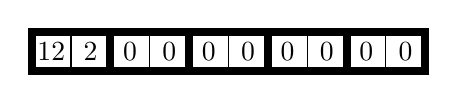
\begin{tikzpicture}[scale=0.5]
  \foreach \x in {0,1,...,9}
    \draw (\x,0) rectangle (\x+1,1);
   \foreach \x/\num in {0.5/12,1.5/2,2.5/0,3.5/0,4.5/0,5.5/0,6.5/0,7.5/0,8.5/0,9.5/0}
     \node at (\x,0.5) {\num};
  \foreach \x in {0,2,...,8}
    \draw[line width=1mm] (\x,0) rectangle (\x+2,1);
\end{tikzpicture}

\end{minipage}
\hspace{5mm}
\begin{minipage}{0.4\textwidth}
\textit{Actual:}
\centering
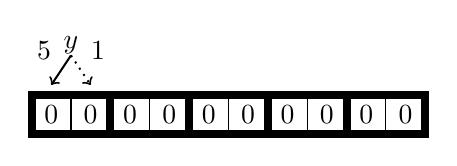
\begin{tikzpicture}[scale=0.5]
  \foreach \x in {0,1,...,9}
    \draw (\x,0) rectangle (\x+1,1);
   \foreach \x/\num in {0.5/0,1.5/0,2.5/0,3.5/0,4.5/0,5.5/0,6.5/0,7.5/0,8.5/0,9.5/0}
     \node at (\x,0.5) {\num};
  \foreach \x in {0,2,...,8}
    \draw[line width=1mm] (\x,0) rectangle (\x+2,1);
  \node at (1.0,2.25) {$y$};
  
  \draw[->, line width=0.25mm] (1.0,2.0) -- node[above left] {$5$} (0.5,1.25);
   \draw[->, dotted, line width=0.25mm] (1.0,2.0) -- node[above right] {$1$} (1.5,1.25);
\end{tikzpicture}
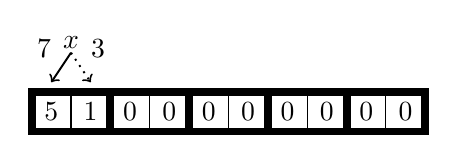
\begin{tikzpicture}[scale=0.5]
  \foreach \x in {0,1,...,9}
    \draw (\x,0) rectangle (\x+1,1);
   \foreach \x/\num in {0.5/5,1.5/1,2.5/0,3.5/0,4.5/0,5.5/0,6.5/0,7.5/0,8.5/0,9.5/0}
     \node at (\x,0.5) {\num};
  \foreach \x in {0,2,...,8}
    \draw[line width=1mm] (\x,0) rectangle (\x+2,1);

  \node at (1.0,2.25) {$x$};
  
  \draw[->, line width=0.25mm] (1.0,2.0) -- node[above left] {$7$} (0.5,1.25);
   \draw[->, dotted, line width=0.25mm] (1.0,2.0) -- node[above right] {$3$} (1.5,1.25);
\end{tikzpicture}
\\[20pt]
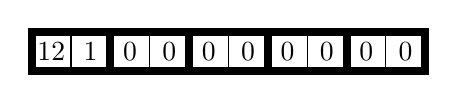
\begin{tikzpicture}[scale=0.5]
  \foreach \x in {0,1,...,9}
    \draw (\x,0) rectangle (\x+1,1);
   \foreach \x/\num in {0.5/12,1.5/1,2.5/0,3.5/0,4.5/0,5.5/0,6.5/0,7.5/0,8.5/0,9.5/0}
     \node at (\x,0.5) {\num};
  \foreach \x in {0,2,...,8}
    \draw[line width=1mm] (\x,0) rectangle (\x+2,1);
\end{tikzpicture}

\end{minipage}

\end{frame}

\begin{frame}{Surprising findings}{Fixing the error}
  \begin{minipage}{0.38\textwidth}
    \centering
    \includegraphics[width=\linewidth]{img/tbf_insertion_pseudo_mark.pdf}
    %\captionof{figure}{fixed pseudocode insertion}
  \end{minipage}
  \hspace{0.1\textwidth} 
  \begin{minipage}{0.38\textwidth}
    \centering
    \includegraphics[width=\linewidth]{img/tbf_insertion_pseudo_fix_mark.pdf}
    %\captionof{figure}{fixed pseudocode lookup}
  \end{minipage}
\end{frame}

\begin{frame}{Surprising findings}{Lookup mistake}
  \begin{minipage}{0.5\textwidth}
    \includegraphics[width=\linewidth]{img/tbf_lookup_text_mark.pdf}
    \captionof{figure}{Description of lookup}
  \end{minipage}
  \begin{minipage}{0.35\textwidth}
    \includegraphics[width=\linewidth]{img/tbf_lookup_pseudo_mark.pdf}
    \captionof{figure}{Pseudocode of lookup}
  \end{minipage}
\end{frame}

\begin{frame}{Surprising findings}{Why?}
    \begin{itemize}
        \item $L=4, k=1, v_{g_{1}{(x)}} = 7, w_{h_{1}{(x)}} = 3$
    \end{itemize}
\begin{minipage}{0.5\textwidth}
\centering
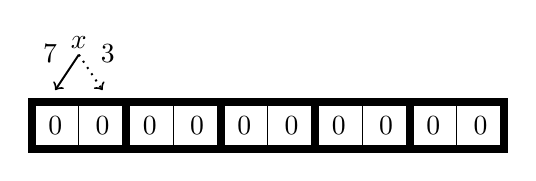
\begin{tikzpicture}[scale=0.6]
  \foreach \x in {0,1,...,9}
    \draw (\x,0) rectangle (\x+1,1);
   \foreach \x/\num in {0.5/0,1.5/0,2.5/0,3.5/0,4.5/0,5.5/0,6.5/0,7.5/0,8.5/0,9.5/0}
     \node at (\x,0.5) {\num};
  \foreach \x in {0,2,...,8}
    \draw[line width=1mm] (\x,0) rectangle (\x+2,1);
  \node at (1.0,2.25) {$x$};
  
  \draw[->, line width=0.25mm] (1.0,2.0) -- node[above left] {$7$} (0.5,1.25);
   \draw[->, dotted, line width=0.25mm] (1.0,2.0) -- node[above right] {$3$} (1.5,1.25);
\end{tikzpicture}

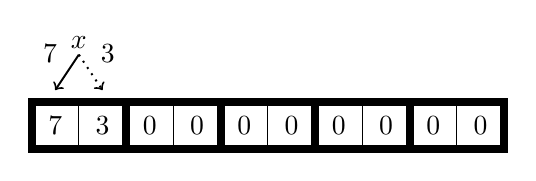
\begin{tikzpicture}[scale=0.6]
  \foreach \x in {0,1,...,9}
    \draw (\x,0) rectangle (\x+1,1);
   \foreach \x/\num in {0.5/7,1.5/3,2.5/0,3.5/0,4.5/0,5.5/0,6.5/0,7.5/0,8.5/0,9.5/0}
     \node at (\x,0.5) {\num};
  \foreach \x in {0,2,...,8}
    \draw[line width=1mm] (\x,0) rectangle (\x+2,1);

  \draw[->, line width=0.25mm] (1.0,2.0) -- node[above left] {$7$} (0.5,1.25);
   \draw[->, dotted, line width=0.25mm] (1.0,2.0) -- node[above right] {$3$} (1.5,1.25);
   \node at (1.0,2.25) {$x$};

\end{tikzpicture}
\\[20pt]
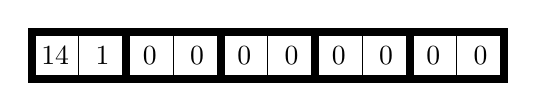
\begin{tikzpicture}[scale=0.6]
  \foreach \x in {0,1,...,9}
    \draw (\x,0) rectangle (\x+1,1);
   \foreach \x/\num in {0.5/14,1.5/1,2.5/0,3.5/0,4.5/0,5.5/0,6.5/0,7.5/0,8.5/0,9.5/0}
     \node at (\x,0.5) {\num};
  \foreach \x in {0,2,...,8}
    \draw[line width=1mm] (\x,0) rectangle (\x+2,1);
\end{tikzpicture}

\end{minipage}
\begin{minipage}{0.35\textwidth}
    \includegraphics[width=\linewidth]{img/tbf_lookup_pseudo_mark.pdf}
\end{minipage}

\end{frame}

\begin{frame}{Surprising findings}{Fixing the error}
  \begin{minipage}{0.38\textwidth}
    \centering
    \includegraphics[width=\linewidth]{img/tbf_lookup_pseudo_mark.pdf}
    %\captionof{figure}{fixed pseudocode insertion}
  \end{minipage}
  \hspace{0.1\textwidth} 
  \begin{minipage}{0.4\textwidth}
    \centering
    \includegraphics[width=\linewidth]{img/tbf_lookup_pseudo_fix_mark.pdf}
    %\captionof{figure}{fixed pseudocode lookup}
  \end{minipage}
\end{frame}


\section{Conclusion}
\begin{frame}{Conclusion}{}
    \begin{itemize}
        \item Enhancement in false positive probability
        \item Increased Complexity $\rightarrow$ overheads in T-CBF
        \item Academic papers aren’t prone to be perfect
    \end{itemize}
\end{frame}

\begin{frame}
  \begin{center}
    \vspace*{\fill}
    
     \textbf{\Huge \textcolor{blue!90!black}{Thank you for your attention!}}
    \vspace*{\fill}
  \end{center}
\end{frame}


\end{document}
